\documentclass{whutmod}
\usepackage{metalogo}
\usepackage{float}
\usepackage{subfigure} 
\usepackage{url}
\usepackage{booktabs}
\usepackage[style=caspervector,backend=biber,utf8]{biblatex}
\addbibresource{wenxian.bib}
\team{23}
\membera{刘子川}
\joba{编程}
\memberb{程宇}
\jobb{建模}
\memberc{陈荣兴}
\jobc{建模}
\hypersetup{
	colorlinks=true,
	linkcolor=black
}

\title{第四次论文格式}
\tihao{4} 

\begin{document}

%	\maketitle
	
	\begin{abstract}
“拍照赚钱”APP 是基于移动互联网的自助式劳务众包平台,使得企业可利 用大众力量,低成本、高效率地完成各种商品检查与信息搜集的任务。本文通过 建立数学模型,就 APP 中的任务定价问题进行分析,给出最优的任务定价方案。
   ~\\%~\\为换行
   
针对问题一, 针对问题的这一段总结。利用什么软件+建立什么模型+算法方法+求解的特点+主要的结果+评价及其推广。  注意黑体字\text{描黑重点关键词}。
~\\

针对问题二,对项目的任务定价规律进行\textbf{定性与定量研究}。利用 Matlab 的 cftool 工具箱绘制出任务的经纬度坐标与定价数据的\textbf{三维拟合图},观察到任务 分布密集的地区任务定价较低。对任务的位置数据进行空间离散化处理和 K-Means 分析,将任务分布的区域等划分为若干网格区域,定义影响任务定价的 四个因子,即网格内任务数量、会员人数、会员平均完成能力、任务与中心点的 距离。运用灰色关联矩阵定量分析四个影响因子与定价的相关度,分别为 0.9710,0.9671,0.9633,0.9390。得出所定义的指标对定价相关性很高,能较好 描述定价规律。最后通过比较未完成任务与已完成任务的相关度矩阵得出距离对 任务的完成的影响是最显著的


针对问题三,
   ~\\
   
针对问题四,
   ~\\

本文中所提到的模型优点主要有两点:一、在与污染源头距离较短时预测抗噪能力较强;二、利用更高定位精度和鲁棒性的直线解析法,溯源追踪能力较强。
  
\keywords{对流扩散方程\quad  直线解析法\quad  溯源算法\quad 拉普拉斯变换\quad }
		
	\end{abstract}
	
	%目录
	\tableofcontents
	\newpage	%换页符
	
	\section{问题重述}	
	\subsection{问题背景}
现代管理中,彼得德鲁克提出了"人力资源"的概念并认为"人力资源是与其他资源不一样的特殊资源",人力资源的其中一个特质是其具有自主流动性。根据勒温的场论,人才会根据自身需求与环境的适应性而做出离开或者留在某个环境的决定。人才是一个城市保持竞争活力和创新力的关键,在世界各国和全国各地积极推出人才吸引的政策背景下,一个地区的人才吸引力的核心内涵就是这个地区所具有的可以影响人才选择的能力。

全面、科学、系统地评价一个城市的人才吸引力是制定人才吸引计划的前提,城市人才吸引评价指标的选取受多方面影响,关键是要符合人才的理想,满足人才的需求和愿望。按照重要程度,人才的需求可以分为发展前景,收入和环境。发展前景是首要关心的因素,收入是人才流动的另一关键因素,环境因素包括治安、交通、污染、教育、医疗、购物等,也都是会考虑的因素。




	
	\subsection{问题提出}
围绕城市地区人才吸引力水平,以城市多指标评价体系为依据,依次提出以下问题:
		 
	\begin{itemize}
	\item [(1)] 根据数学模型及收集的数据,定量地分析武汉市的人才吸引力水平,并就武汉市的人才政策对人才吸引力水平的影响作出定量评价。
	\item [(2)] 结合人才类别,针对不同类型的人才,深入分析比较武汉市与其他同类城市在人才吸引力上的优势与不足,并给出有效提升人才吸引力的可行方案。
	\item [(3)] 结合模型结果及分析,给武汉市人力资源管理部分写一篇建议报告,要求论点明确,论据充分。
	\end{itemize}
	
	\section{模型假设}
	\begin{itemize}
		\item [(1)] 就写假设就行了吧
		\item [(2)] 
		\item [(3)]
		\item [(4)]
	\end{itemize}
	
	
	\section{符号说明}
%	每行都有线的表
%	\begin{center}
%		\begin{tabular}{cc}
%			\hline
%			\makebox[0.3\textwidth][c]{符号}	&  \makebox[0.4\textwidth][c]{意义} \\ \hline
%			$C_{0}$	    &  污染源初始浓度 \\ \hline
%			$C(x,t)$	    &  污染浓度随时空变化 \\ \hline
%			$u_{x}$	    &  江河平均纵向流速 \\ \hline
%			$E_{x}$  &  铊在江河纵向弥散系数\\ \hline
%		$p$   &  面污染物纵向距离\\ \hline
%			$K_{c}$	    & 污染物降解系数  \\ \hline
%		    $a$	& 污染超标系数 \\ \hline
%		     $x$	& 距污染源的一维距离 \\ \hline
%		      $t$	& 距污染发生后的时间 \\ \hline
%		       $V_{A}$	& 溶液摩尔体积 \\ \hline
%		      $M_{B}$	& 江水的摩尔质量 \\ \hline
%		     $\mu_{B}$	& 溶剂的粘度 \\ \hline		      
%		\end{tabular}
%	\end{center}

%三线表
	\begin{table}[H]
	\label{biao} \centering
		\begin{tabular}{cccc}
			\toprule[1.5pt]
			\multicolumn{1}{m{4cm}}{\centering 符号} & \multicolumn{1}{m{4cm}}{\centering 说明} & \multicolumn{1}{m{4cm}}{\centering 单位}\\
			\midrule[1pt]
			$C_{0}$	 &  污染源初始浓度 & 单位\\ 
			$C(x,t)$ &  污染浓度随时空变化 & 单位\\ 
			$u_{x}$	 &  江河平均纵向流速 & 单位\\ 
			$E_{x}$  &  铊在江河纵向弥散系数& 单位\\ 
			\bottomrule[1.5pt]
		\end{tabular}
	\end{table}

	\section{问题一模型的建立与求解}
	\subsection{问题的描述与分析}

	针对问题一,本题要求对武汉的人才吸引力做出量化评价。对于人才吸引力水平模型,现在主要存在的问题是定性研究较多、量化评价较少,对变量之间的关系讨论更是不足。本文采用因子分析法建立模型,将通过不同的因子对变量的影响程度进行分析,建立客观的评价模型。首先根据题目要求和以往人才吸引要素研究,寻找合适的人才吸引力因素,确立要素框架并寻找各个因素相对应的数据。在将所得数据进行无量纲化处理后,进行$KMO$检验和巴特利特检验以验证所选变量是否适合做因子分析。通过主成分分析法确定公因子数目,求解旋转后因子荷载矩阵并对公因子命名,最后在对武汉各年人才吸引力做出综合得分,其流程图如图\label{llll}所示:


	\begin{figure}[H]
		\centering
		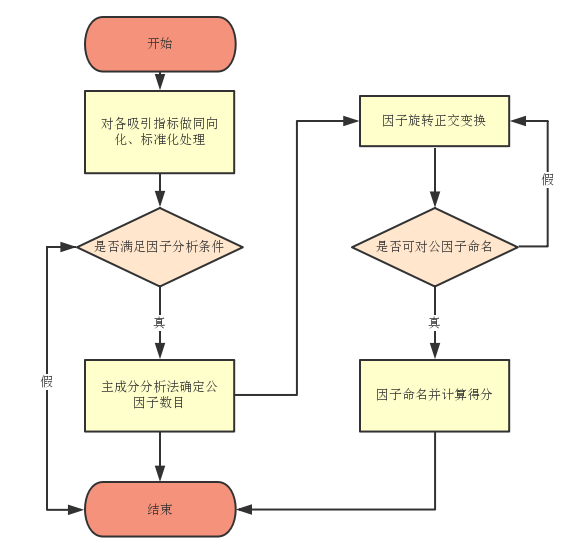
\includegraphics[width=\textwidth]{figures/1111.png}
		\caption{因子分析算法流程图}\label{llll}
	\end{figure}

		\subsection{预备工作}
		\subsubsection{评价指标体系构建}
		参考国家统计局对人才标准的划分,此处对人才的界 定是指,具有大专及以上学历的人员,以及具有初级以上 专业技术职称的人员或在专业技术岗位上工作的人员。
		
		在构建武汉市人才吸引力评价指标体系时,在指标方面,若选取总量太多,在评价模型时太为复杂,可行性低,若数据太少则评价不够准确,脱离实际性。因此为尽可能客观反映吸引力,我们在遵循建立指标体系的科学性、系统性、可操作性、可比性原则\parencite{lepawsky2010metropolis},并兼顾总量指标和相对指标,选取城市发展前景、主要行业收入、政府影响、环境因素、年末总人口共5个二级指标和33个三级指标,多维度、全方面的考虑各个指标对人才吸引力的影响。具体指标体系如图~\ref{lct}~所示: 	
		\begin{figure}[H]
			\centering
			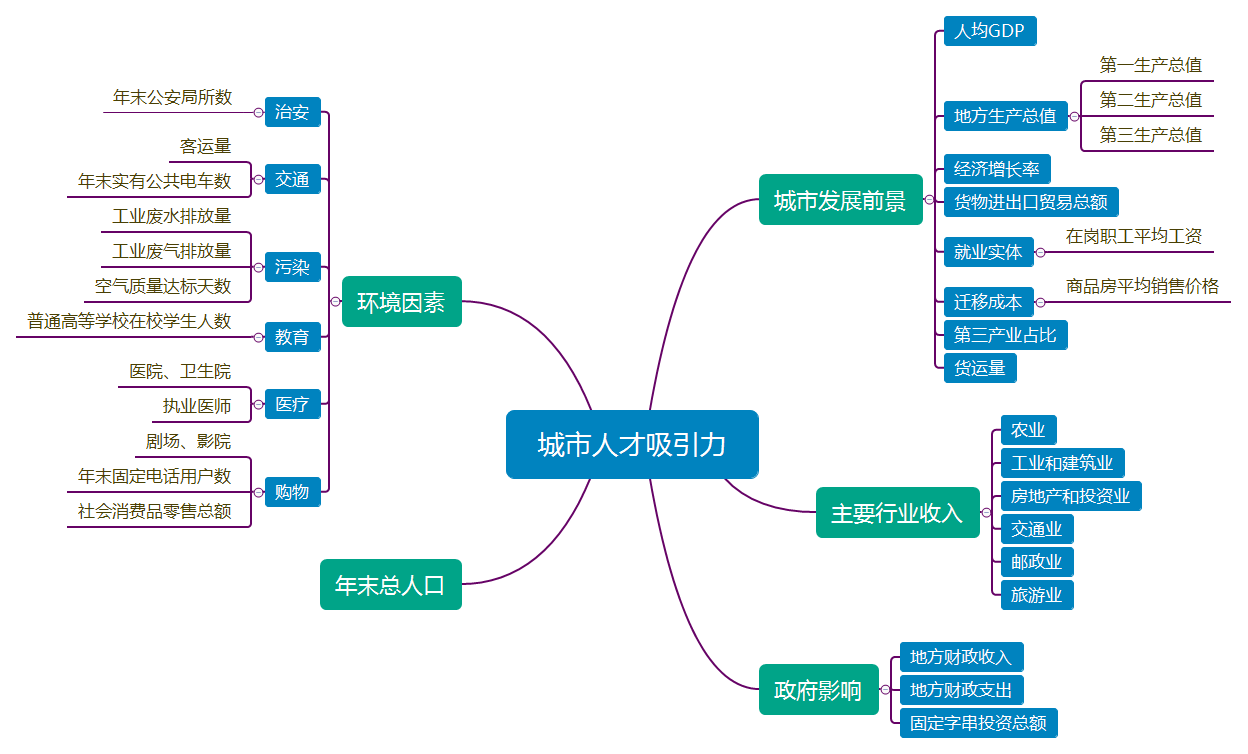
\includegraphics[width=\textwidth]{figures/clt.png}
			\caption{城市人才吸引力指标体系}\label{lct}
		\end{figure}  
		
		\subsubsection{同向化处理}

		在评价城市人才的指标中,工业废水废气排放量和商品房平均销售价格不是越高越好,为方便比较,对这三个指标进行同向化处理\parencite{张瑞红2012河南省产业集群环境人才吸引力评价研究}, 公式如下:
		\begin{gather}
		\widetilde{X}=-(X-\overline{X})
		\end{gather}
		式中:$X$原始指标,$\overline{X}$为原始指标$X$的平均值,$\widetilde{X}$为同向化指标。
		
		\subsubsection{标准化处理}
		为了对变量进行比较并消除由于观测量纲的差异及数量级差异所造成的影响,将样本观测数据进行标准化处理,使标准化的变量均值为$0$,方差为$1$。其处理方法如下:
		\begin{gather}
		Z=\frac{X-\overline{X}}{\delta_{X}}
		\end{gather}
		式中:$\overline{X}$为$X$的均值,$\delta_{X}$是$X$的标准差。
		
		\subsubsection{KMO与Bartlett检验}
		根据标准化处理后的指标数据,利用$SPSS23.0$统计软件进行$KMO$和巴特利特检验,以确认所选变量是否适合做因子分析,结果如表\label{tab1}所示:
		% Table generated by Excel2LaTeX from sheet 'Sheet1'
		\begin{table}[H]
			\centering
			\caption{KMO和Bartlett的检验}\label{tab1}
			\begin{tabular}{cc|cc|cc}
				\toprule[1.5pt]
				\multicolumn{4}{c|}{取样足够度的Kaiser-Meyer-Olkin度量} & \multicolumn{2}{c}{0.859} \\
				\midrule
				\multicolumn{2}{c|}{\multirow{3}[2]{*}{Bartlett的球形度检验}} & \multicolumn{2}{c|}{近似卡方} & \multicolumn{2}{c}{1183.981} \\
				\multicolumn{2}{c|}{} & \multicolumn{2}{c|}{df} & \multicolumn{2}{c}{78} \\
				\multicolumn{2}{c|}{} & \multicolumn{2}{c|}{Sig.} & \multicolumn{2}{c}{.000} \\
				\bottomrule[1.5pt]
			\end{tabular}%
			\label{tab:addlabel}%
		\end{table}%
		
		由上表可知,巴特利特球度检验统计量的观测值为$1183.981$,相应的概率$P$值接近$0$。若显著性水平$α$为$0.5$,概率$P$小于显著性水平$α$,应拒绝零假设,认为相关系数矩阵与单位阵有显著差异,即因子协方差矩阵不是单位阵。同时,$KMO$值为$0.859$,$KMO>0.8$,根据$KMO$ 度量标准可知原有变量适合进行因子分析。
		
		
		

	\subsection{模型的建立与求解}
	\subsubsection{公因子的确定}
	标准化后数据如表一所示(附表一),表一相关系数矩阵$R$如下(附加相关系数矩阵)
	设$\lambda_{1} \geqslant \lambda_{2} \geqslant \cdots \geqslant \lambda_{p}$为样本相关系数矩阵$R$的特征值,$\eta _ { 1 } , \eta _ { 2 } , \cdots , n _ { p }$为相应的标准正交化特征向量。设$m<p$,则因子载荷矩阵$\Lambda$为:
	\begin{gather}
	\Lambda=\left[\sqrt{\lambda_{1}} \eta_{1}, \sqrt{\lambda_{2}} \eta_{2}, \cdots, \sqrt{\lambda_{m}} \eta_{m}\right]
	\end{gather}
    用$\boldsymbol{R}-\boldsymbol{\Lambda} \boldsymbol{\Lambda}^{\mathrm{T}}$对角元来估计特殊因子的的方差
	\begin{gather}
	\sigma_{i}^{2}=1-\sum_{j=1}^{m} \alpha_{i j}^{2}
	\end{gather}
	得总方差解释如表三(附表三)
	
	
	
	由表$3$特征根知,因子$1$的特征值$λ1=25.330$,占方差的 $76.75\%$。由图$1$知,当提取$1,2$个公因子时,特征值变化非常明显,当提取第$5$个以后的公因子时,特征值变化比较小,基本趋于平缓。由此说明,提取$4$个公因子对原变量信息的刻画有显著作用。因此,在这里我们提取$4$个公共因子,这$4$个公因子的累计方差达到$99.92\%$,即这$4$个公因子可以反映原来$33$个指标的$99.92\%$的信息量,可见采用前$4$个公因子对武汉2013——2017年人才吸引力进行评价是比较合适的。
	
	\subsubsection{未转轴的因子载荷矩阵}
	表 4 中的每个数据表示了相应因子变量对相应原变量的相对重要程度。由于得到的公共因子与各指标的载荷分布归类比较困难,需要对因子载荷矩阵进行正交旋转,这里运用方差最大正交旋转法,得到旋转后的因子载荷矩阵表(4)。
	表$3$是初始因子载荷矩阵,由此可写出因子分析模型的如下:
	\begin{gather}
	\begin{array} { l } { \mathrm { X } _ { 1 } = 0.989 \mathrm { F } _ { 1 } + 0.123 \mathrm { F } _ { 2 } - 0.074 \mathrm { F } _ { 3 } - 0.031 \mathrm { F } _ { 4 } } \\ { \mathrm { X } _ { 2 } = 0.795 \mathrm { F } _ { 1 } - 0.556 \mathrm { F } _ { 2 } - 0.193 \mathrm { F } _ { 3 } - 0.151 \mathrm { F } _ { 4 } } \\ { \ldots \ldots } \\ { \mathrm { X } _ { 33 } = - 0.958 \mathrm { F } _ { 1 } + 0.176 \mathrm { F } _ { 2 } - 0.060 \mathrm { F } _ { 3 } + 0.220 \mathrm { F } _ { 4 } } \end{array}
	\end{gather}
	通过凯撒正态化最大方差法,旋转在$9$次迭代后已收敛。得表$5$(附表五)
	
	根据表$5$发现,旋转后的因子系数已经明显向两极分化,有了更鲜明的实际意义。因子载荷的绝对值越大,则表明该因子与变量的重叠性越高,在解释因子的时候就越重要。
	(因子命名)
	\subsubsection{求得因子得分和综合绩效得分}
	采用回归法估计因子得分系数,并输出因子得分系数矩阵。具体结果见表$6$
	由估计出的因子得分,可以量化描述城市人才吸引力水平,利用因子得分可以从不同角度对城市人才吸引力水平进行比较分析。为了便于对各城市进行人才吸引力评价,现利用武汉每年的因子得分表计算综合得分,吸引力水平的获取是基于总方差分解表中旋转后各因子的方差贡献率及计算所得的城市各因子得分获取的。其计算公式如下:
	\begin{gather}
	\mathrm { F } = \left( 55.267 \mathrm { F } _ { 1 } + 17.845 \mathrm { F } _ { 2 } + 14.623 \mathrm { F } _ { 3 } + 12.265 \mathrm { F } _ { 4 } \right) / 99.92
	%(附结果计算公式)
	\end{gather}
	计算结果见表$7$
	\subsection{结果分析}
	
	\section{问题二模型的建立与求解}
	\subsection{问题的描述与分析}
	问题二要求针对具体人才类别,量化分析比较武汉市与其它同类城市的人才吸引力。本文在问题一模型的基础上改进,将人才分为三个阶段————初级人才、中级人才和高级人才,并将问题一中的人才吸引力因素分为针对各发展阶段人才的主要影响因素,再对分类后数据进行因子分析得到成都、天津、西安、南京和武汉$2013~2017$年分别对于三类人才吸引力的因子分析模型。
	\subsection{模型的建立与求解}
	\subsubsection{人才的分类}
	人才在不同发展阶段会有不同的关注焦点,所以城市对不同	发展阶段的人才吸引力影响因素也存在差异。我们把人才分为三个阶段:初级人才、中级人才和高级人才。收集成都、天津、西安、南京和武汉对应问题一中的人才吸引力要素,并将收集的因素归类为对各发展阶段人才的主要影响因素。如表$8$所示:
	(表8)
	\subsubsection{分级人才吸引力分析}
	将归类后所得的影响低级人才吸引力的$??$个影响因素在五个城市中$2013~2017$年的数据,使用SPSS进行因子分析,按照累积贡献率的原则提取公因子,以综合性指标来相对全面的反映出全体因子对初级人才吸引力的影响情况。按照主因子的提取原则,很明显地看出可以用$??$个主因子来描述此$??$个因子的影响。然后得出主因子的解释方差解释如表9所示:
	表(9)
	通过表$9$中的方差贡献率及计算所得的城市各因子得分得到各城市每年的初级人才吸引力综合得分。其计算公式如下:
	\begin{gather}
	\mathrm { F } = \left( 55.267 \mathrm { F } _ { 1 } + 17.845 \mathrm { F } _ { 2 } + 14.623 \mathrm { F } _ { 3 } + 12.265 \mathrm { F } _ { 4 } \right) / 99.92
	%(附结果计算公式)
	\end{gather}
	将得到的五个城市$2013~2017$年的综合得分绘制为折线图的到图(1)如下所示
	图(1)
	同理将归类后所得的影响中级人才吸引力的$??$个影响因素使用SPSS进行因子分析,得到方差解释表如表10所示
	(表10)
	得到中级人才吸引力综合得分计算公式:
	\begin{gather}
	\mathrm { F } = \left( 55.267 \mathrm { F } _ { 1 } + 17.845 \mathrm { F } _ { 2 } + 14.623 \mathrm { F } _ { 3 } + 12.265 \mathrm { F } _ { 4 } \right) / 99.92
	%(附结果计算公式)
	\end{gather}
	中级人才吸引力综合得分折线图:
	图(2)
	
	同理高级人才吸引力的$??$个影响因素因子分析得得方差解释表如表11所示
	(表11)
	
	高级人才吸引力综合得分计算公式:
	\begin{gather}
	\mathrm { F } = \left( 55.267 \mathrm { F } _ { 1 } + 17.845 \mathrm { F } _ { 2 } + 14.623 \mathrm { F } _ { 3 } + 12.265 \mathrm { F } _ { 4 } \right) / 99.92
	%(附结果计算公式)
	\end{gather}
	高级人才吸引力综合得分折线图:
	\subsection{结果分析}
	%时间分析
	由图表可以看出对XX人才吸引力逐年上涨···
	%地域分析 
	由人才吸引力这一简单的方面可以反映我国西部和东部的综合实力差异和自然环境造成的优劣。可以说,人才吸引力的评价就是综合实力评价的缩影版。
	%综合分析



%	\parencite{geng2019novel}为文献引用
	查阅资料可得\parencite{宋鸿2010城市人才吸引力的影响因素及提升对策}
	
%	~\ref{llllll}~为图表引用,中间为为图表\label{}
具体浓度分布如图~\ref{llllll}~所示:


	\section{问题二模型的建立与求解}
	\subsection{问题的描述与分析}
%	问题分析写\textbf{流程图!!}其流程图如图~\ref{lct}~所示:
%			\begin{figure}[H]
%	\centering
%	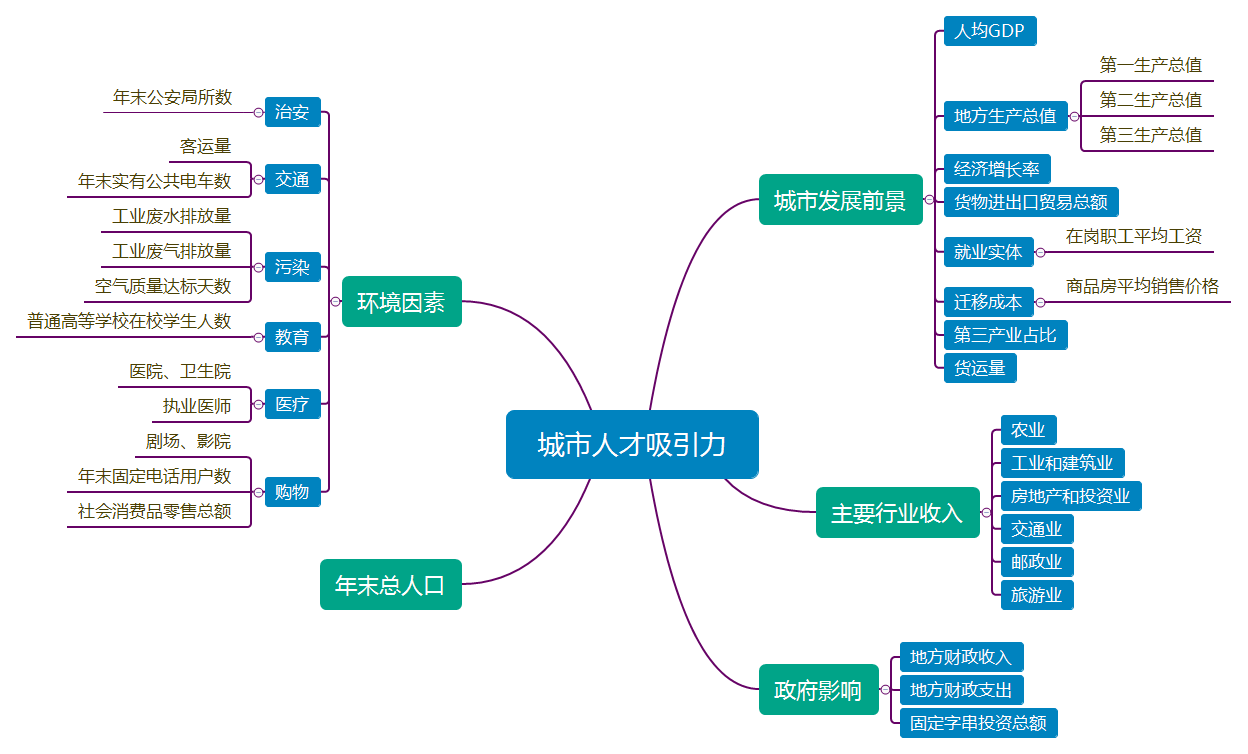
\includegraphics[width=.8\textwidth]{figures/clt.png}
%	\caption{算法流程图}\label{lct}
%	\end{figure}
	\subsection{模型的建立与求解}
	

	\section{问题三的求解}
	
	
	\subsection{写给武汉市人力资源部门的建议报告}
	
武汉市人力资源管理部分的领导:

武汉市作为全国科技和教育事业最发达的地区之一, 无论在拥有高校数量还是毕业生质量方面都位居前列。就业政策体系不断完善,扶持就业创业力度不断加大,社会保障体系建设取得突破性进展,人才队伍建设卓有成效。随着”黄鹤英才计划”,”3551人才计划”等重大人才工程的推进,累计引进,培养中央”千人计划”、国家”万人计划”、省”百人计划”等顶尖人才375人,吸纳引进海内外高层次创新创业人才4000余人,数量居中部城市第一。

人才决定着一个城市的发展前景, 但城市必须拥有足够的吸引力才能让人才流入。人才在选择移居城市时必然会去对这个城市进行量化评估并与其他城市进行对比, 进而去选择最适和发展的城市。发展前景,迁移成本、薪资待遇以及城市各方面环境因素、政府策略都是会是考虑的因素。我们只有紧紧抓住人才这个关键环节,才能在新一轮经济发展和城市竞争中取得优势,因此我们建立了人才吸引力影响因素和政策效力的模型,在政策制定有很大的理论和现实意义,并向贵部门提出相关建议。

通过以2017年国家统计年鉴和2017年各大城市统计年鉴和各式人力资源和社会保障局官网的相关数据为依据,对以武汉市在内的同类型城市(西安、成都、天津、南京、武汉)人才吸引力水平进行分析。我们结合了因子分析法和主成分分析法地代数模型进行研究,首先构建评价指标体系。遵循客观地、科学性和系统性地原则选取了城市发展前景、主要行业收入、政府影响、环境因素、年末总人口共5个二级指标和33个三级指标。并应用因子分析将33个三级指标综合成4个公共因子,这4个公因子的累计方差达到$99.2\%$。用这4个公因子来对武汉城市吸引力进行评价,再利用主成分分析法提取,构建未转轴的因子载荷矩阵,得到因子的分析模型后,进行正交旋转,对两级分化的因子系数进行命名,第一个主因子包含xxxxxxx,第二个主因子包含xxxxxxxxx, 第三个主因子包含xxxxxxxxx ,第四个主因子包含xxxxxxxxx。多次旋转迭代后的成分矩阵已收敛,得到最终的人才吸引力评价模型,计算各因子的作用权重,并给出五座城市的综合排名。研究数据表明………………………………


在本次研究中,武汉市的城市基础设施建设、经济发展状况………….


因此,针对以上情况我们向有关领导提出以下建议
加强基础设施建设,提升西安市的生活环境、公共卫生医疗的服务水平。加大社会保障力度,加强公共交通的便利程度,提升人均住房 面积,完善人才引进资金补贴和创业基金补助。加快“一带一路”发展进程,在经济发展中找寻机遇,提高软实力 的竞争性。完善人才引进政策,购房优惠政策、落户门槛降低、提供更多的个人发展机会。完善人才评价机制,提 高工作积极性,促进激励政策。“内留外引”政策,提高武汉本地毕业生的留用率,留住本地人才。



本研究还存在一些局限性,本研究的数据均来源于各类统计年鉴和人力资源和社会保障厅官网,受数据的限制,尚有其他相关重要的测量指标数据未能获取,仅能 得到相对条件下的相对结论,使得本研究与现实情况之 间出现一些偏差,未来或需引入一些新的能够容纳更多信息的方法。




	\section{模型的评价}
	\subsection{模型的优点}
xxxxxxxxxxxxxxxxxxxxxxxxx
	
	\subsection{模型的缺点}
xxxxxxxxxxxxxxxxxxxxxxxxxxxxxx


	\subsection{模型的改进与展望}%
xxxxxxxxxxxxxxxxxxxxxxxxxxxx
	\newpage	%换页符
	%%参考文献
	%\begin{thebibliography}{9}%宽度9
	% \setlength{\itemsep}{-2mm}
	\nocite{*}		%排版未引用的参考文献
	\printbibliography[title = {参考文献}]	%使用国标参考文献添加方式
	%参考文献添加到wenxian.bib里,再引用
	
	\newpage
	%附录
	\appendix %%附录
\section{代码}
\subsection{爬取数据--python源代码}
\begin{lstlisting}[language=python]%这里修改语言
xxxxxxxxxxxxxxxxxxxxxxxxxxxxxxxx
\end{lstlisting}

\end{document}